% setup the document and include packages
\documentclass{article}[12pt]
\usepackage{graphicx}
\usepackage{amsmath}
\usepackage{amssymb}
\usepackage{cancel}
\usepackage{ntheorem}
\usepackage{algorithm2e}
\usepackage{float}
\usepackage{caption}
\usepackage{fancyvrb}
\usepackage[dvipsnames]{xcolor}
\usepackage[section]{placeins}
\usepackage[toc,page]{appendix}
\usepackage{hyperref}

%set stuff for syntax highlighting
\usepackage{fontspec}
\usepackage{minted}
\setsansfont{Calibri}
\setmonofont{Consolas}

\newcommand{\comment}[1]{}

\hypersetup{
    colorlinks=true,
    linkcolor=blue,
    filecolor=magenta,      
    urlcolor=cyan,
}
\urlstyle{same}

\makeatletter
\def\BState{\State\hskip-\ALG@thistlm}
\makeatother

\makeatletter
\g@addto@macro\@floatboxreset\centering
\makeatother

% define Continue for algorithms
\SetKw{Continue}{continue}

% Define custome verbatim command to insert maze text file results
\RecustomVerbatimCommand{\BVerbatimInput}{VerbatimInput}%
{fontsize=\footnotesize,
 %
 frame=lines,  % top and bottom rule only
 framesep=2em, % separation between frame and text
 rulecolor=\color{Black},
 %
 %label=\fbox{\color{Black}data.txt},
 labelposition=topline,
 %
 %commandchars=\|\(\), % escape character and argument delimiters for
                      % commands within the verbatim
 %commentchar=*        % comment character
}

% redefine QED symbol
\renewcommand{\qedsymbol}{\rule{0.7em}{0.7em}}

% define lemma and result theorem-styled sections
\newtheorem{lemma}{Lemma}[section]
\newtheorem{result}{Result}[section]

% Don't print the semicolon in algorithms
\DontPrintSemicolon

% define the title that will be used in the report
\title{CS 598 PS \\ Machine Learning for Signal Processing \\ Problem Set 3}
\author{
Christian Howard \\ howard28@illinois.edu
}
\date{} % don't set a date because we don't need this shit


% setup paths for images
\graphicspath{ {../scripts/} }

% start the document
\begin{document}
   
   % create the title page 
   \maketitle
   \begin{abstract}
   	Within this report is a set of solutions for Problem Set 3 spanning areas of classification. In the first two parts of the problem set, theoretical and practical efforts were made related to Gaussian discriminant functions. On the theoretical side, discriminant functions were derived based on Baye's Rule and Gaussian assumptions on the conditional distribution for input data. On the practical side, it was found that Gaussian discriminant functions could achieve up to a 91\% classification success rate using PCA features in $\mathbb{R}^{26}$. The third part of this problem set revolved around classification of different sounds. By formulating the input as a stack of frequency information for 1 second worth of time samples, the input data was reduced using a randomized projection to a dimension of $\mathbb{R}^4$. Cross-validation found an average 93.8\% classification success rate using a Gaussian discriminant classifier. Additionally, this classifier correctly classified custom recordings passed into it. The last part of this problem set revolved around classification of pools in satellite styled imagery. Using Gaussian discriminant functions once again, three Gaussians were learned to represent pool, building, and the ground distributions and classify if some pixel is a part of either distribution. Using this classifier, a sample test image was passed into the classifier and produced a fairly accurate classification of the pools located in the image.
   \end{abstract}
   \newpage
   
   % create table of contents on separate page
   \tableofcontents
   
   
   \newpage
   \section{Part 1 - Discriminant Function Theory}
   The goal of this problem is to derive formulations for Gaussian discriminant functions and then use them to plot the discriminant functions for a set of sub-problems, each with a set of two Gaussian distributed classes with given means and covariances. Taking a look at the theory first, we know that a fundamental idea to this approach is to take some distribution for a class, $\omega$, and compute the probability that a class is valid for some input, $x$. We can write this out using Baye's Rule as the following:
   
   \begin{align*}
    P(\omega | x) &= \frac{P(x | \omega) P(\omega)}{P(x)}
   \end{align*}

   Given we have a set of classes, we can then find the class that best represents some input $x$ through the below computation:

   \begin{align}
   \omega^* &= \arg \max_{\omega_k} P(\omega_k | x) \nonumber \\
   &= \arg \max_{\omega_k} P(x | \omega_k) P(\omega_k) \nonumber \\
   &= \arg \max_{\omega_k} \log\left(P(x | \omega_k)\right) + \log\left( P(\omega_k) )\right) \nonumber \\
   &= \arg \max_{\omega_k} g_k(x) \label{eq:maxg}
   \end{align}

   where $\omega^*$ is the best class representing the input $x$ and $g_k(\cdot)$ is the discriminant function for an associated class $\omega_k$. If we then assume that $P(x|\omega_k)$ can be modeled as a Gaussian and that $P(\omega_k)$ is known, then we can readily compute the above classification. First, a multivariate Gaussian model can be defined as the following for some $x \in \mathbb{R}^n$:

   \begin{align*}
    P(x) &= \frac{
    	e^{-\frac{1}{2} \left(x - \mu\right)^{T} \Sigma^{-1}\left(x - \mu\right) }
    }{\sqrt{(2\pi)^{n} |\Sigma|}} 
   \end{align*}
   
   where $\mu$ is the expected value for $x$ and $\Sigma$ is the coveriance for $x$. If we use a multivariate model for some class $\omega_k$, we can derive the below discriminant function:

   \begin{align*}
    g_k(x) &= \log\left(P(x | \omega_k)\right) + \log\left( P(\omega_k) )\right) \\
    &= \frac{-n}{2} \log\left(2\pi\right) - \frac{1}{2}\log|\Sigma_k| - \frac{1}{2} \left(x - \mu_k\right)^{T} \Sigma_k^{-1}\left(x - \mu_k\right) + \log\left( P(\omega_k) )\right) \\
    &= \lbrace \log\left( P(\omega_k) )\right) - \frac{n}{2} \log\left(2\pi\right) - \frac{1}{2}\log|\Sigma_k| - \frac{1}{2} \mu_k^{T} \Sigma_k^{-1} \mu_k \rbrace + \mu_k^{T} \Sigma_k^{-1} x - \frac{1}{2} x^{T} \Sigma_k^{-1}x \\
    &= a_k + b_k^T x + x^{T} C_k x \\
   \end{align*}

   where $a_k  = \lbrace \log\left( P(\omega_k) )\right) - \frac{n}{2} \log\left(2\pi\right) - \frac{1}{2}\log|\Sigma_k| - \frac{1}{2} \mu_k^{T} \Sigma_k^{-1} \mu_k \rbrace$ is a scalar, $b_k = \Sigma_k^{-1} \mu_k$ is a vector, and $C_k = - \frac{1}{2} \Sigma_k^{-1}$ is a matrix. Also note that $\mu_k$ and $\Sigma_k$ represent the expected value and covariance for $x$ given we are in class $\omega_k$. One last point is that since the input $x$ will be the same dimension for all the discriminants, the $\frac{n}{2} \log\left(2\pi\right)$ term in $a_k$ is not actually needed. 

   With this closed form for the discriminant, all that needs to be done to define the discriminant function is computing the expected value and covariance for $x$ for each class' set of data. Given that is complete, using (\ref{eq:maxg}) we can compute the class some input is best represented by. For $x \in \mathbb{R}^2$, we can also visualize the discriminant function boundary by plotting $f(x) = g_1(x) - g_0(x)$ and finding where $f(x) = 0$. Figures \ref{fig:dpa}, \ref{fig:dpb}, \ref{fig:dpc}, and \ref{fig:dpd} show the discriminant decision boundaries and Gaussian distributions for Parts a, b, c, and d for this problem based on their provided Gaussian hyperparameters. In general, the decision boundaries make sense, though the boundary for Part c, found in Figure \ref{fig:dpc}, is not super obvious due to the distributions sitting on top of each other. Due to that, I found the decision boundary for Part c interesting to observe.

	\begin{figure}[ht]
		\centerline{
			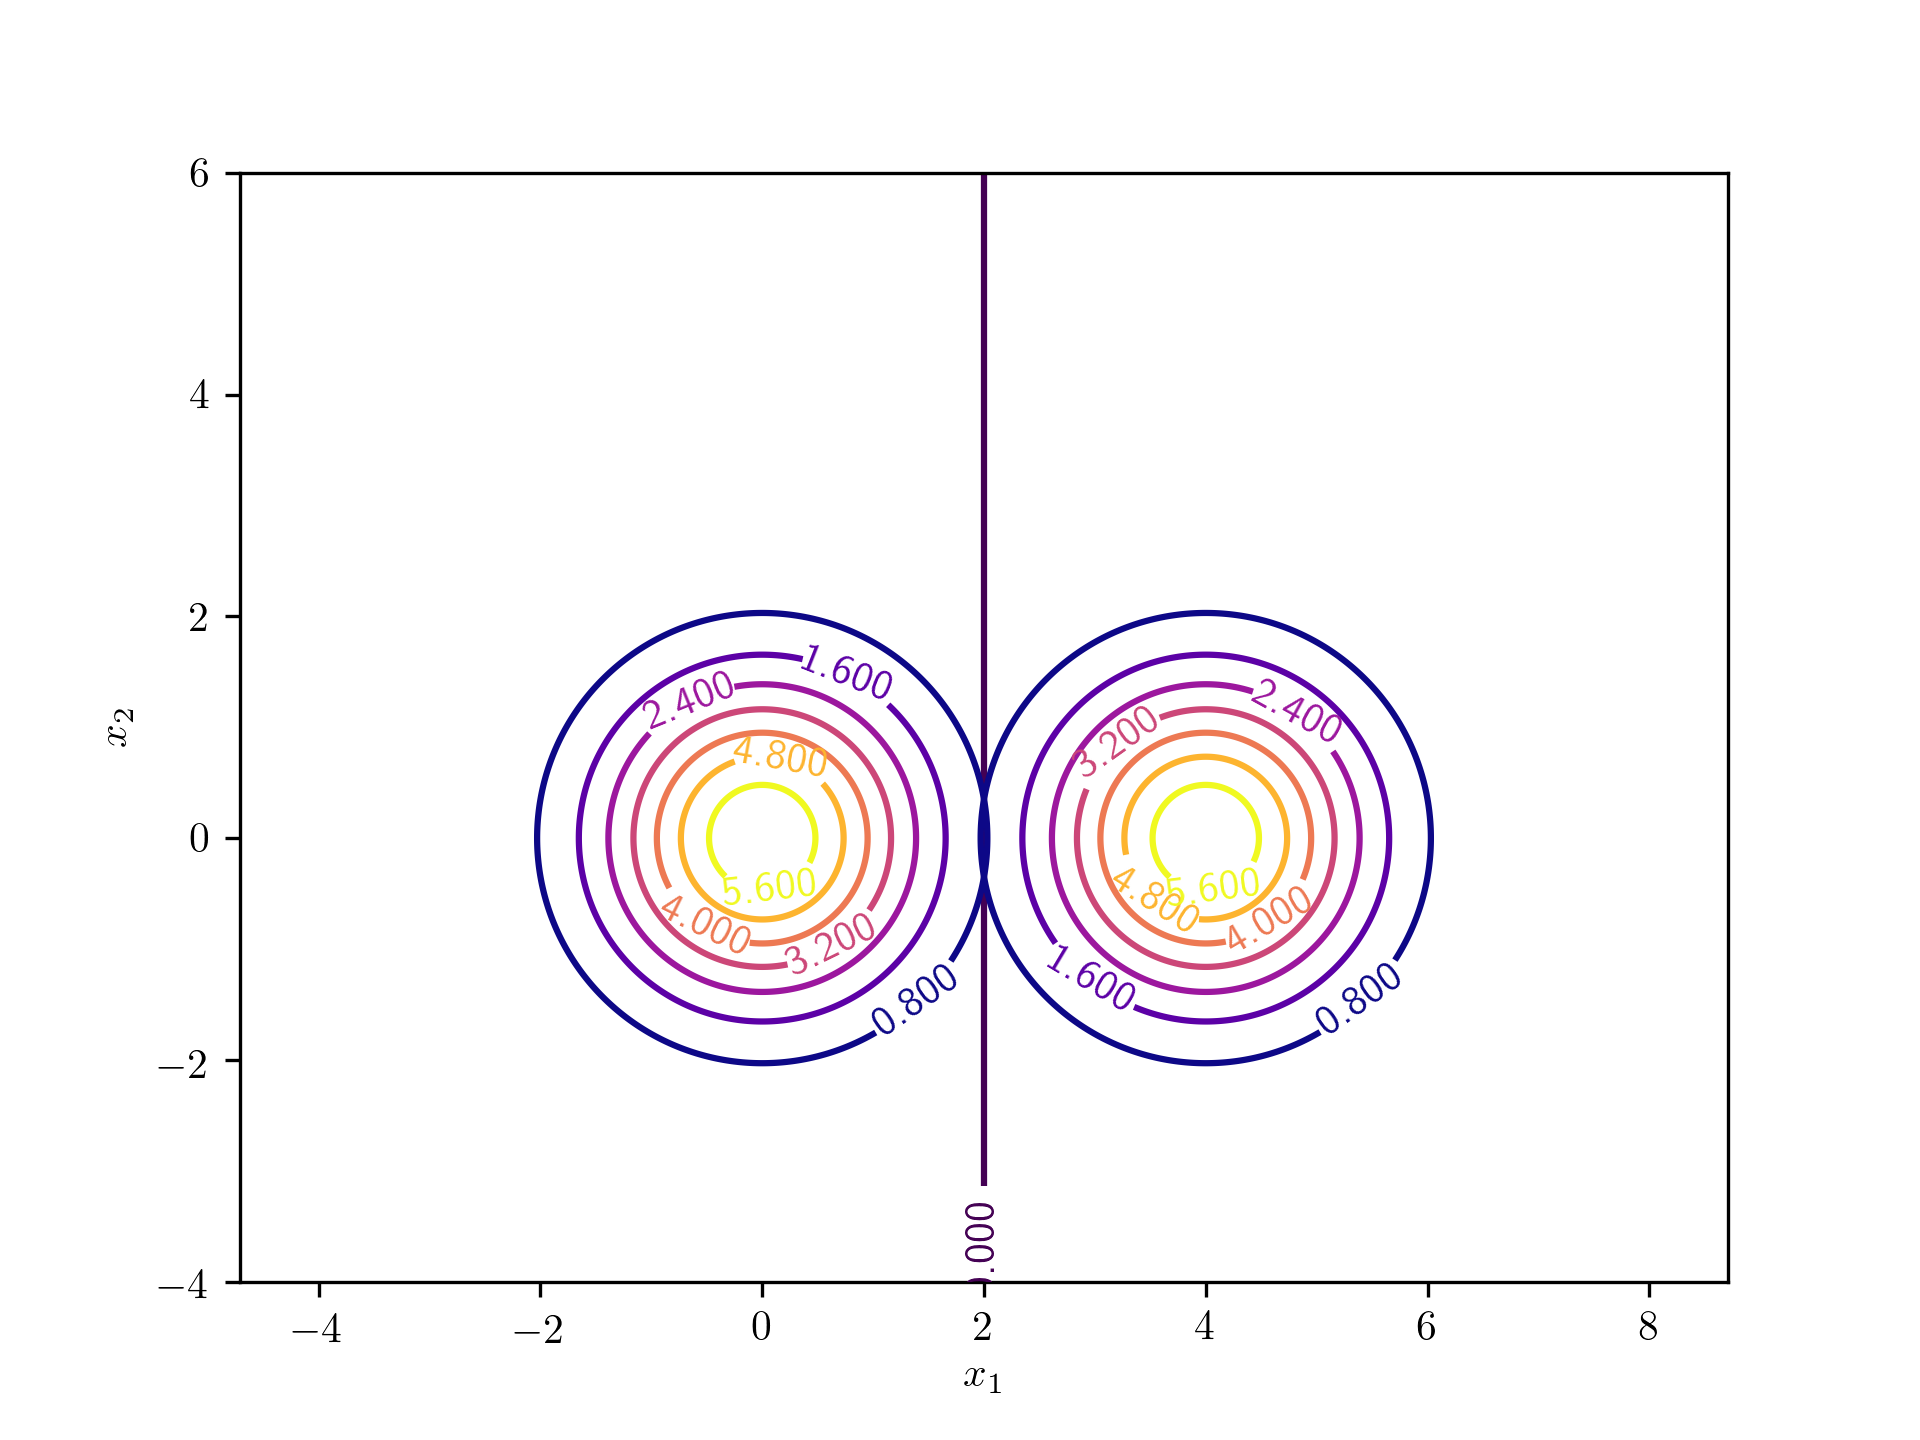
\includegraphics[scale=0.7]{../scripts/p1/discriminant_a.png}}
		\caption{Discriminant for Part a}
		\label{fig:dpa}
	\end{figure}

\begin{figure}[ht]
	\centerline{
		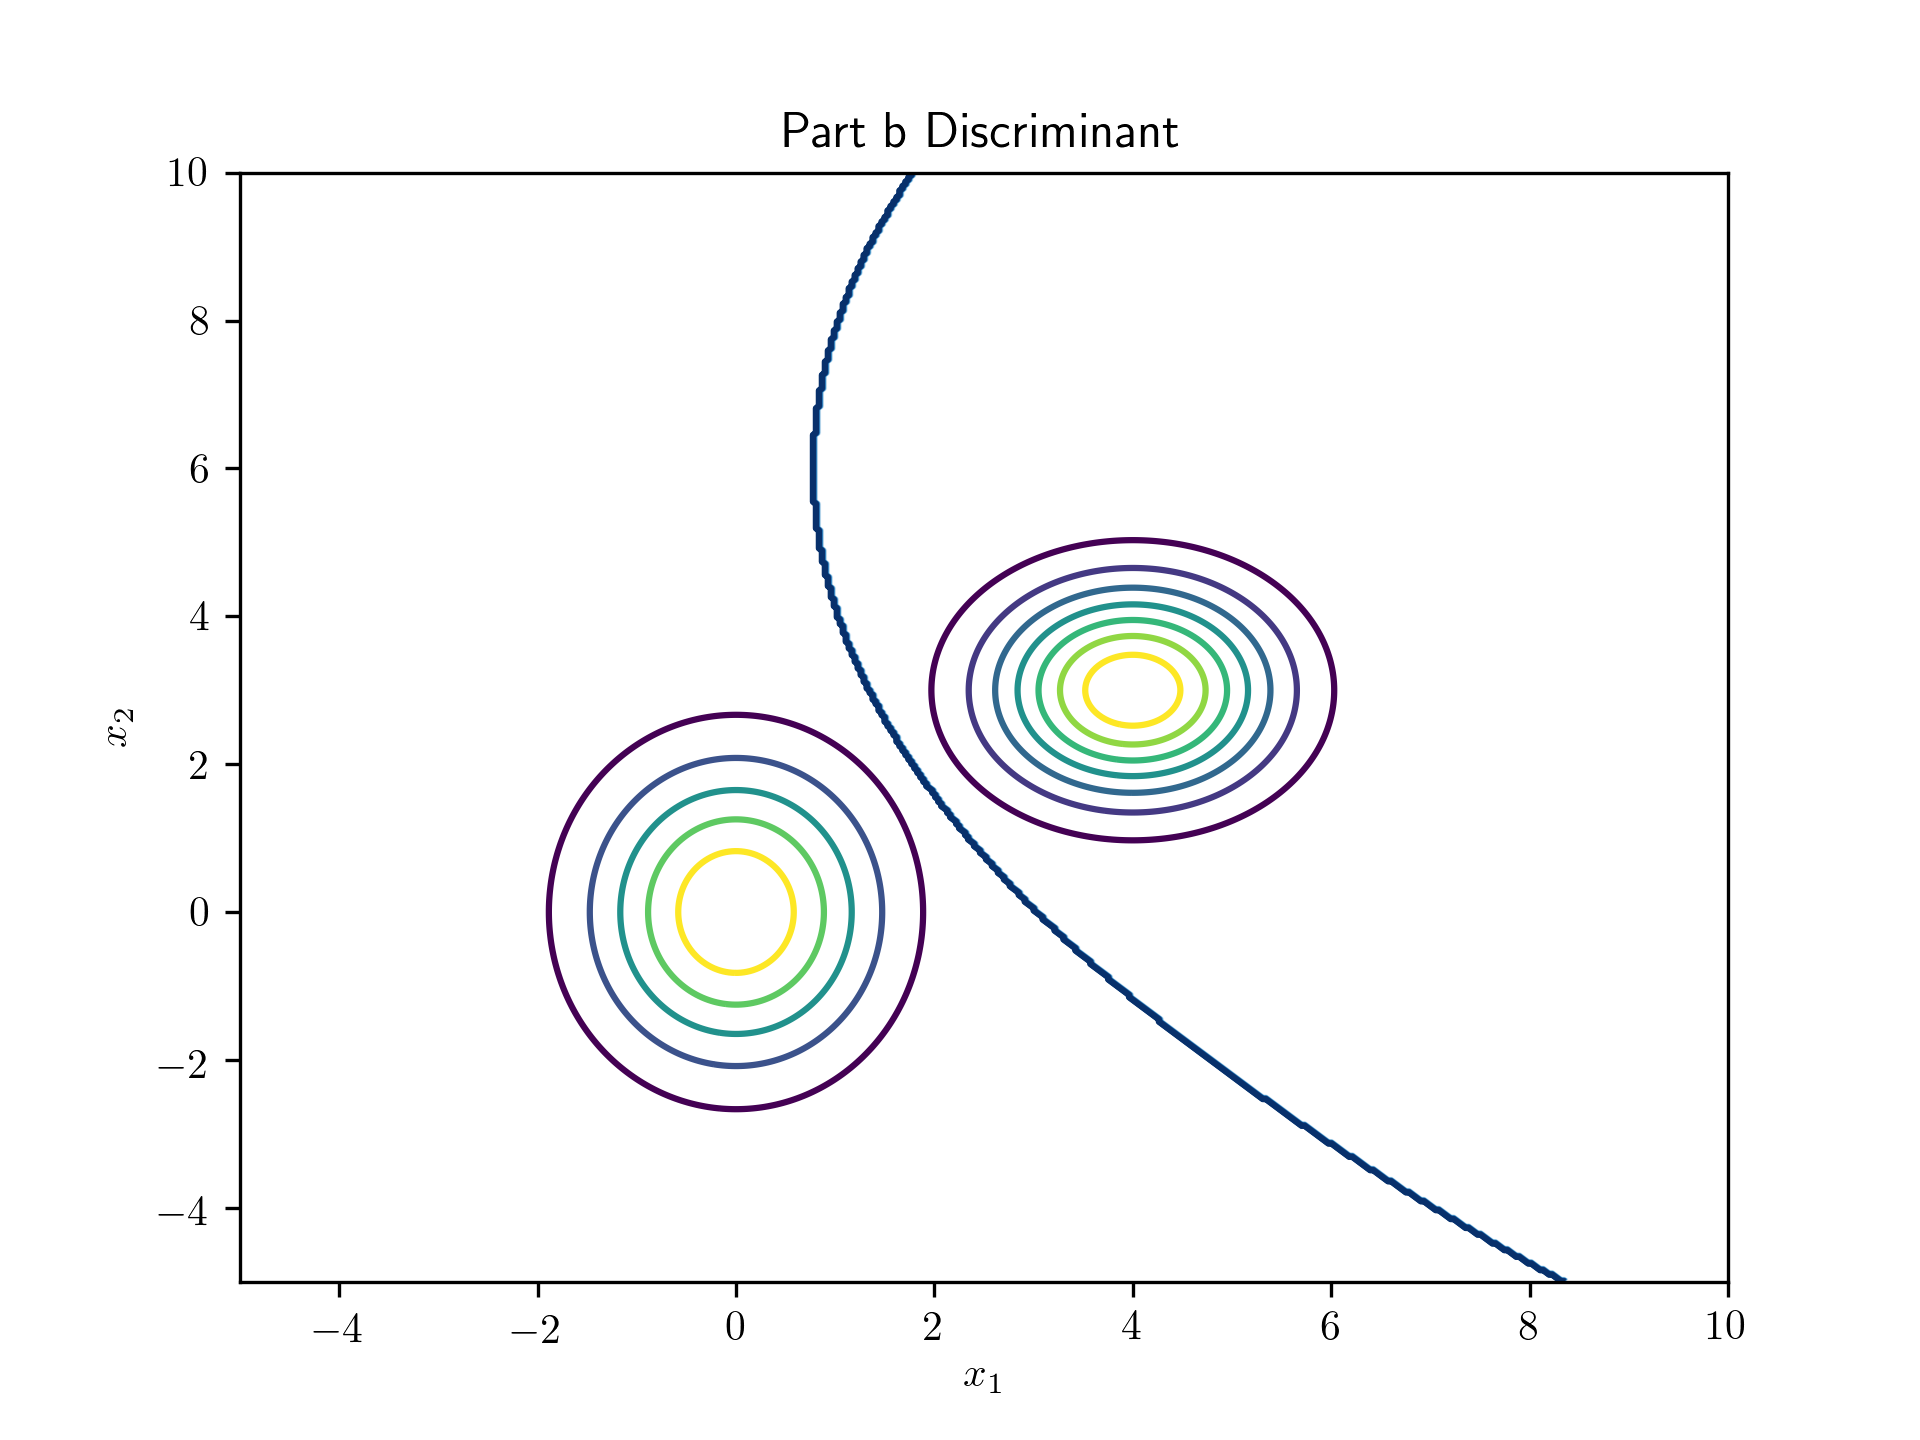
\includegraphics[scale=0.7]{../scripts/p1/discriminant_b.png}}
	\caption{Discriminant for Part b}
	\label{fig:dpb}
\end{figure}


\begin{figure}[ht]
	\centerline{
		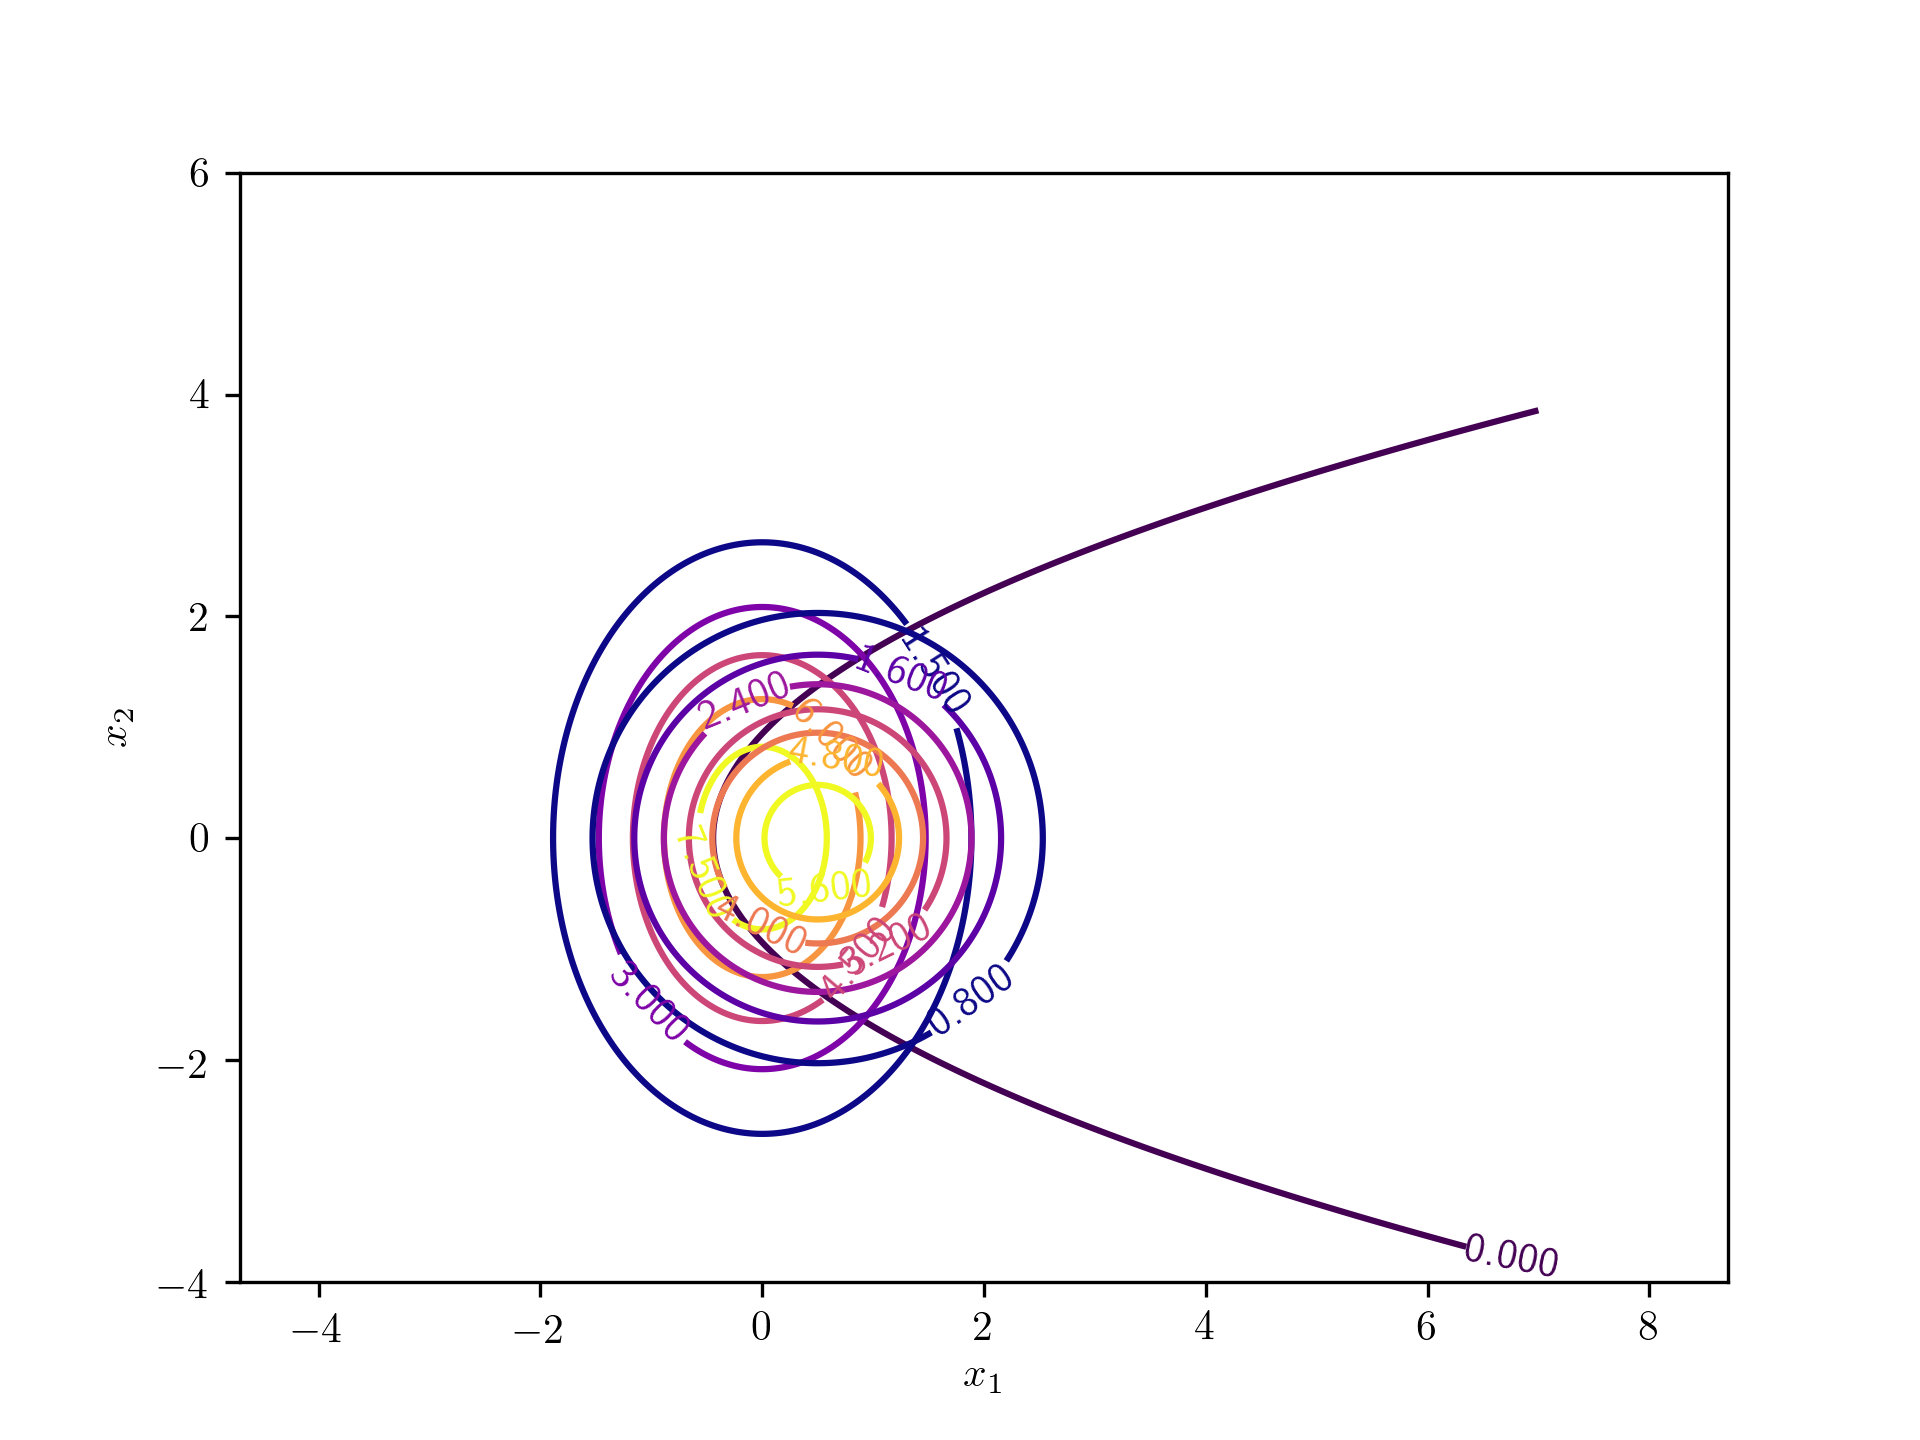
\includegraphics[scale=0.7]{../scripts/p1/discriminant_c.png}}
	\caption{Discriminant for Part c}
	\label{fig:dpc}
\end{figure}


\begin{figure}[ht]
	\centerline{
		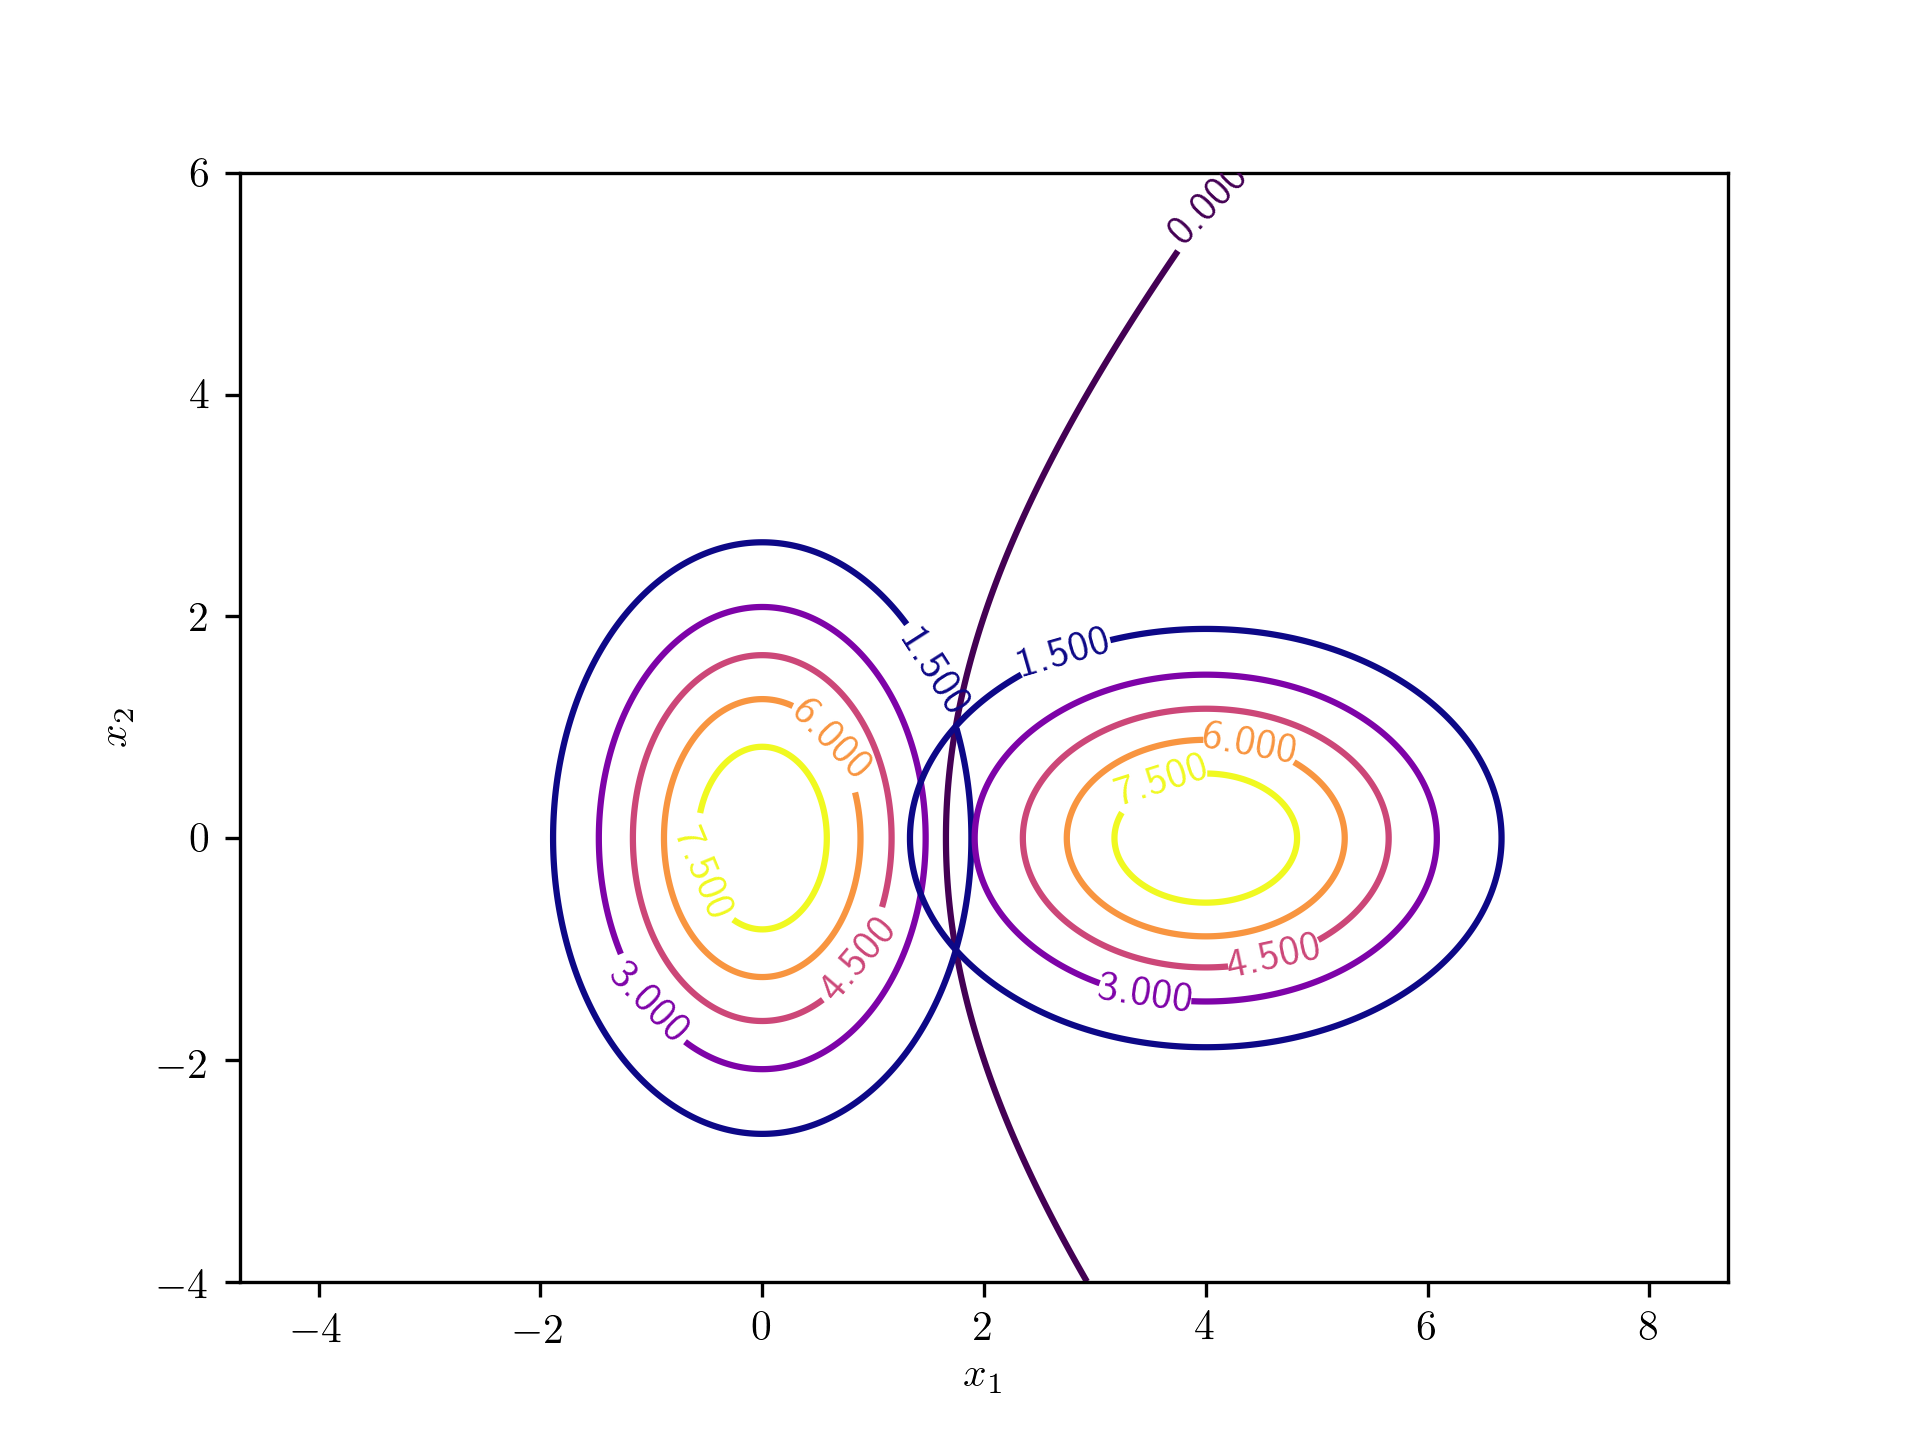
\includegraphics[scale=0.7]{../scripts/p1/discriminant_d.png}}
	\caption{Discriminant for Part d}
	\label{fig:dpd}
\end{figure}

\newpage
   \section{Part 2 - Discriminant Functions in Practice}
   Within this problem, we are tasked to classify hand written digits using Gaussian discriminant functions. Our constraints were that we must use 100 digits of data for each class to train the classifier and then use the rest of the data for testing.

   Now with my implementation of Gaussian discriminant functions and my randomized PCA algorithm, it was found that I needed to drop the dimensionality of the input data from $\mathbb{R}^{784}$ to $\mathbb{R}^{33}$ to achieve greater than a 90\% classification success rate. The features for this reduced dimensionality are shown in Figure \ref{fig:p2ftrs}. One thing I will note is that I found features based on the whole dataset. One interesting pattern I noticed was that if my dimensionality got too high, the classification rate actually performed worse. 
   
   Part of this appears to be due to bad conditioning of the covariance matrices formed at these higher dimensions, since I wrote my code to try to form the full covariance estimate. In fact, I had times where the covariance matrices were singular for some digits, given some specified dimension reduction, while other digits did not produce singular covariances for the same dimension reduction. This implied that some digits did not have enough variation for a given lower dimensional representation, which made things interesting.

\begin{figure}[ht]
	\centerline{
		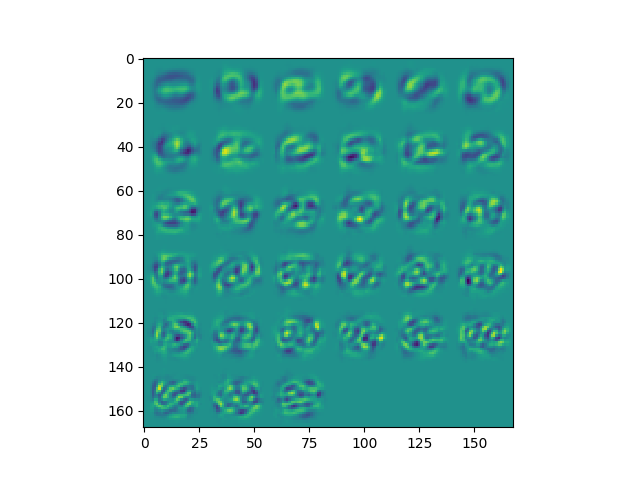
\includegraphics[scale=0.7]{../scripts/p2/resulting_features.png}}
	\caption{Features for Dimensionality achieving 90\% Classification Success}
	\label{fig:p2ftrs}
\end{figure}

   It was also found that if I reduced the dimensionality too much, it appears not enough information was provided to best distinguish between classes because the classification performance struggled here as well. It became obvious there was more of a sweet spot, a range for the dropped dimensionality that would perform more favorably in the classification task. To make this a little easier for myself, I just used a bisection algorithm to find the dimensionality that hovered around a 90\% classification success rate, which happened to be finding features that reduced the data to 33 dimensions. The best classification success rate found for the testing data was 91\% using features with 26 dimensions.

	\newpage
   \section{Part 3 - Classifying Speech versus No Speech}
   Within this part of the problem set, we were tasked to come up with a classifier that could distinguish between speech and music given a provided dataset of recordings. Additionally, we were tasked to perform a cross-validation estimate of how good the classification model performs by using 90\% of the data each experiment to train and the rest to test. 
   
   After performing cross-validation across 1000 experiments, permuting what data was used to train and test for each experiment, it was found that on average 93.8\% of the classifications made were correct. Additionally, this classifier correctly classified the recordings I provided, each with their spectrograms defined in Figures \ref{fig:srec} and \ref{fig:mrec}. 
   
   \begin{figure}[ht]
   	\centerline{
   		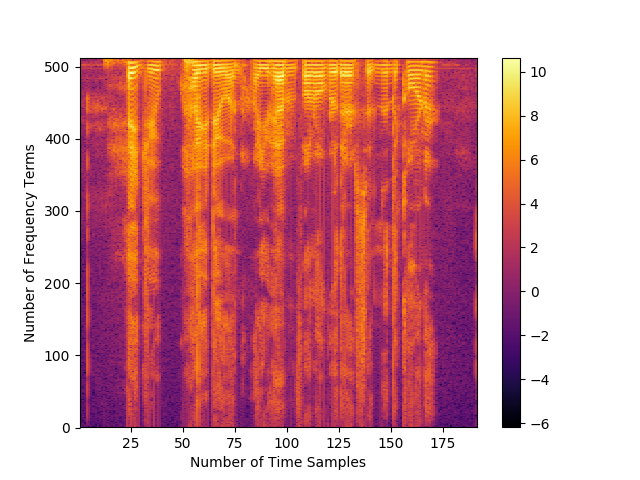
\includegraphics[scale=0.5]{../scripts/p3/spectrogram_speech.png}}
   	\caption{My Speech Recording}
   	\label{fig:srec}
   \end{figure}

	\begin{figure}[ht]
		\centerline{
			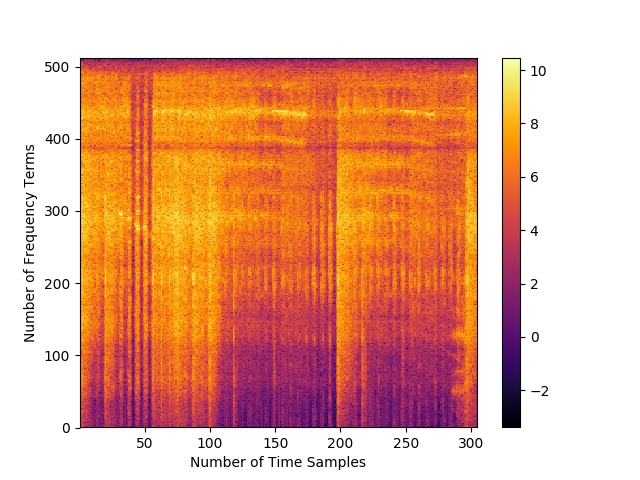
\includegraphics[scale=0.5]{../scripts/p3/spectrogram_music.png}}
		\caption{My Music Recording}
		\label{fig:mrec}
	\end{figure}

   To tackle this problem, I first defined an input as about 1 second worth of spectrogram data generated with a window size of 1024 samples and a hopsize of 512 samples. I then took each recording and sliced their respective spectrograms into 1 second chunks, labeled according to if it was speech or music, and brought all of this into a dataset. Since the sounds were recorded at 22,050 Hz, I found that the closest chunk of samples I could get to being one second was 21,504 samples, meaning that some sample from my input data $X \in \mathbb{R}^{21,504}$. This being a huge dimensionality, I used my randomized projection algorithm to reduce the dimensionality from $\mathbb{R}^{21,504}$ to $\mathbb{R}^{4}$. Note that this 4 dimensional data representation was found empirically to perform well.
   
   With that new dimensionality, building and evaluating the Gaussian Classifiers was simple using my code for Gaussian discriminant functions. After recording myself speaking and a sound playing off of my phone, I just loaded in those sounds with the proper sampling rates, turned their data into the desired 1 second spectrogram chunks, and tested it against my classifier. 

   I want to note that my first approach actually did not treat inputs as 1 second chunks, instead evaluating 1 second worth of the the original spectrogram inputs and finding which classification was most common and labeling that 1 second chunk accordingly. It worked but I ditched that for the above method because I felt that my first attempt might not take into account any transient relationships that might exist over a 1 second time frame. 

	\newpage
   \section{Part 4 - Classification of Pools}
   In this part for the problem set, it is our goal to build a model that can learn to identify pools using some input training image and then detecting pools in images passed to it. The solution I found to this problem was once again using Gaussian discriminants. In this instance, I did not perform any dimensionality reduction because the three color components should already be minimal dimensions for representing variance in inputs from an arbitrary satellite image of some region. 
   
   \begin{figure}[ht]
   	\centerline{
   		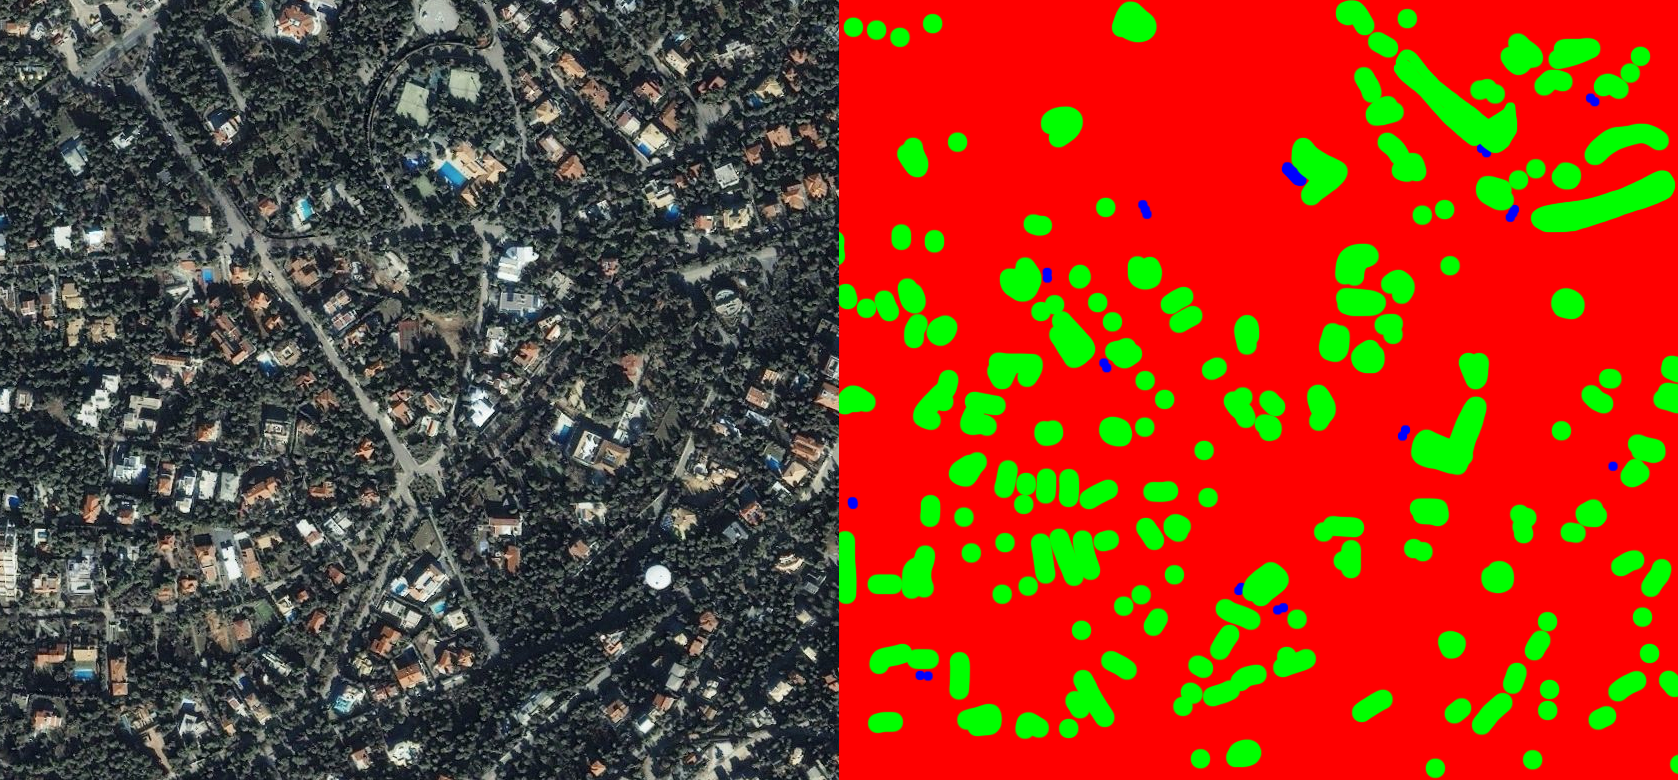
\includegraphics[scale=0.3]{img/p4_train_data_compare.png}}
   	\caption{Training Data. Left represents input image provided and Right represents Labels painted based on provided input. Colors represent labels for \textcolor{blue}{pools}, \textcolor{green}{buildings}, and the \textcolor{red}{ground}}
   	\label{fig:ptrain}
   \end{figure}

   Additionally, in the end I chose to model this problem using three Gaussians, the classes being pools, buildings, and the ground. I arrived at these classes after first trying to use purely pool versus non-pool classes. Trying to tackle this problem using the two classes resulted in some obvious classification errors, which I suspected might be due to larger variances in the non-pool class Gaussian since this Gaussian was based on lighter colored buildings and darker colored ground. After changing to three models, the classification results were much better behaved for identifying pools. Figure \ref{fig:ptrain} shows the inputs to the algorithms used to build the model and Figure \ref{fig:pdetect} shows the before and after pool classification results for the test image. 
   
   As we can see by taking a look at Figure \ref{fig:pdetect}, most, if not all, of the more obvious pools were classified and marked appropriately. There were also some areas that could be pools, but lighting from the image make it a little tough to know for sure. While there was some spurious classification errors, in general the classifier performed pretty well based on inspecting the test image.
   
   I want to also mention some of my initial (failed) attempts to solve this problem using some form of clustering. I worked out codes for $k$-means and spectral clustering but found the following issues. First, $k$-means seemed to never arrive at means that were sufficiently close to an expected value for a color that might represent a pool. I have a suspicion part of the issue is because the pool related colors could almost be viewed as outliers when compared to the overall color point cloud. This means that with so many pixels, the pool related colors were likely smoothed out via computing means for each subset. Even if there was a good way to use the resulting clusters for classification after the fact, the cluster means were not adequate.
   
   With respect to spectral clustering, I was hoping that perhaps the affinity matrix would help to produce better clusters based on distance relationships between colors in the point cloud. Two issues came up with this approach. First, the dataset was too large to actually use in construction of the affinity matrix given I made no assumption on the sparsity of the affinity matrix. Second, it was not obvious how I could use any resulting features to cluster and eventually classify data from a new dataset. 
   
   After thinking enough about the above too methods, I realized Gaussian discriminants were really the basis for what I was after anyway, so that is what lead me to a usable solution.

   \begin{figure}[ht]
   \centerline{
   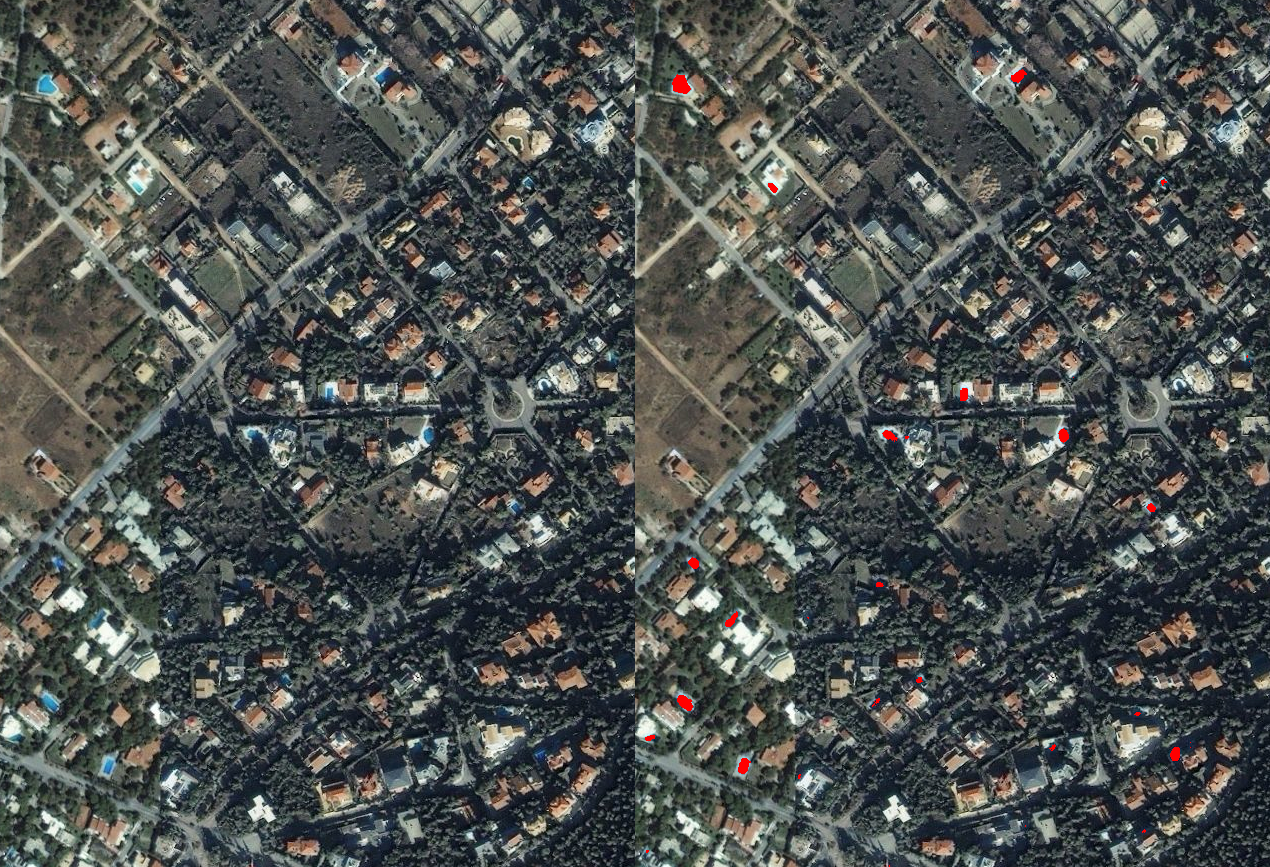
\includegraphics[scale=0.4]{img/p4_soln_compare.png}}
   \caption{Pre-Detection vs. Pool Detection (Pools in \textcolor{red}{Red})}
   \label{fig:pdetect}
   \end{figure}

\newpage
  \section{Project Proposal}
   As a proposal for the final project, Sameer Manchanda, Ryley Higa, and myself would like to work together with a goal of taking a large, existing functional magnetic resonance imaging (fMRI) dataset and using it to discover some insightful transient features in the brain and then building a set of non-parametric models, one using deterministic methods and one using probabilistic methods. 
   
   We base our modeling on the idea that there may be simple cognitive processes (which would be discovered by feature extraction) that vary in change in activation level over time (modeled by multiplicative weights that vary over time).  The deterministic model would be based on a non-parametric regression approach to modeling the weights (as we believe the behavior would likely be nonlinear), while the probabilistic model would be based on assuming the weights are distributed according to a rectified linear Gaussian process, which could be approximated using variational inference. For the variational inference, we would first develop a model using a mean field formulation (meaning we approximate the posterior by assuming variational factors are independent). 
   
   As a stretch goal, we would strive to improve the approximation by relaxing the mean-field assumption. Given we can find adequate models via variational inference, we would then be interested in differences between the non-parametric regression model and variational inference models. We see the main steps of difficulty as the following:
   
   \begin{enumerate}
   	\item Adequately reduce the neuroscience dataset to a manageable size using dimensionality reduction techniques and seeing what insight we can gain into the features extracted. Challenges with this area is the size of the data. It is feasible we could reduce the data by thinning the spatial point cloud, be it randomly, by zooming in to some region of the brain, or some other strategy. If we opt to use the complete dataset, it is possible custom algorithms would need to be built. This could entail the development of some distributed algorithms just to reduce the dimensionality of the data to something manageable.
   	\item The intermediate work would be to develop the the non-parametric regression and rectified linear Gaussian process (using mean field variational inference) models. We could then compare these models and arrive at any pros and cons using each.
   	\item The stretch goal would be to remove some of the assumptions posed by the mean field formulation to variational inference and coming up with a new model that is still feasible to compute. Ideally we could get to a point computing this model and comparing it to the models in part 2.
   \end{enumerate}
   
   
   \newpage
   \section{Software Used}
   The following libraries were used to help with opening data files, algorithm development, and post-processing:
   
   \begin{itemize}
   \item numpy
   \item matplotlib
   \item scipy
   \end{itemize}

	No Machine Learning libraries were used in this problem set.
   
   \newpage
   \section{Specialized Software Written}
   Code was written in this problem set for Gaussian discriminant functions, $k$-means, spectral clustering via affinity matrices, and then utility functions used like a Bisection code and code for breaking up datasets into training and testing chunks. Any library type codes written by me can be found in any Python package directory starting out with \textbf{my}, an example being \textbf{myml/}. Below is the source for some of these new codes.
   
   
   \begin{minted}[mathescape,
               linenos,
               numbersep=5pt,
               gobble=2,
               frame=lines,
               framesep=2mm]{python}
      # import important libs
      import numpy as np
      import scipy as sp
      import scipy.sparse
      import myml.factorizations as myfac

      def evalKMeans(X, means):
          # Author: Christian Howard
          # Code to compute what cluster some input data is 
          # input means found via k-means associated with 
          # based on distance from

          (d, nd) = X.shape
          idx = np.zeros((1,nd),dtype=int)

          # assign mean to each coordinate
          for k in range(0, nd):
              delta = np.linalg.norm(means - X[:, k].reshape(d,1), axis=0)
              idx[0,k] = np.argmin(delta)

          # return the output index list
          return idx



      def spectral(X, distfunc, num_means, max_iter = 1e3, tol = 1e-3, print_msg = False):
          # Author: Christian Howard
          # Method to perform spectral clustering via an 
          # Affinity Matrix formulation, given some distance 
          # function and the number of clusters you're looking for

          # get dimensions of data
          (d,nd) = X.shape

          # construct affinity matrix
          if print_msg:
              print('Starting construction of affinity matrix')
          A = np.zeros((nd,nd))
          Dv = np.zeros((nd,1))
          for i in range(0,nd):
              for j in range(0,nd):
                  if i != j:
                      A[i,j] = distfunc(X[:,i],X[:,j])
              Dv[i] = 1.0/np.sqrt(np.sum(A[i,:]))
              if print_msg:
                  print('Finished row {0} out of {1} in construction'.format(i+1,nd))

          if print_msg:
              print('Finished Creation of nominal Affinity Matrix')

          # construct normalized affinity matrix
          Dm = sp.sparse.spdiags(Dv,0,nd,nd)
          An = Dm@A@Dm

          if print_msg:
              print('Finished Creation of Normalized Affinity Matrix')

          # do PCA on the affinity matrix
          (Q,Z) = myfac.projrep(An,k_or_tol=d,num_power_method=10)
          W = Q.T

          if print_msg:
              print('Finished dimensionality reduction')

          # do kmeans on the resulting data Z
          means = kmeans(Z, num_means=num_means,
                            max_iter=max_iter,
                            tol=tol,
                            print_msg=print_msg)

          if print_msg:
              print('Finished kmeans')

          # do cluster classification
          return evalKMeans(Z, means)



      def kmeans(X, num_means, max_iter = 1e3, tol = 1e-3, print_msg = False):
          # Author: Christian Howard
          # Function to perform k means on some input dataset X

          # initialize kmeans variables
          (d,nd)  = X.shape
          idx0    = np.random.choice(nd,size=num_means,replace=False)
          means   = X[:,idx0]
          means0  = np.copy(means)
          err     = 1e3
          iter    = 0

          # do k means EM algorithm
          indices = np.zeros((1,nd),dtype=int)
          while iter < max_iter and err > tol:

              # assign cluster
              for k in range(0,nd):
                  delta       = np.linalg.norm(means - X[:,k].reshape(d,1),axis=0)
                  indices[0,k]= np.argmin(delta)

              # update means
              for k in range(0,num_means):
                  means[:,k] = np.mean(X[:,np.where(indices==k)[1]],axis=1)

              # compute change in means
              err = np.linalg.norm(means - means0)
              means0[:,:] = means[:,:]

              # print message
              if print_msg:
                  print('After {0} iterations, change in means is {1}'.format(iter,err))

              # update iteration count
              iter += 1

          # return the means
          return means
\end{minted}

\begin{minted}[mathescape,
linenos,
numbersep=5pt,
gobble=2,
frame=lines,
framesep=2mm]{python}
  import numpy as np
  import math
  import myml.factorizations as myfac

  def getGaussianDiscriminantParams(mean, covariance,ProbOmega):
      # Author: Christian Howard
      # Function to get Gaussian discriminant function parameters given
      # some mean, covariance, and probability of some class

      invC = np.linalg.inv(covariance)
      Wm = -0.5*invC
      Wv = invC@mean
      ws =  -0.5*(mean.T@Wv) 
            - 0.5*np.log(np.linalg.det(covariance)) 
            + np.log(ProbOmega)
      return (Wm, Wv, ws, invC)

  def evalGaussianDiscriminant(x, discrParams ):
      # Author: Christian Howard
      # Function to compute a gaussian discriminant given some input X
      # and a tuple with the discriminant parameters

      Wm = discrParams[0]
      Wv = discrParams[1]
      ws = discrParams[2]
      return (x.T.dot(Wm)*x.T).sum(axis=1) + Wv.T.dot(x) + ws

  def evalGuassianPDF(x, mean, cov, inv_cov):
      # Author: Christian Howard
      # Function to evaluate a Gaussian PDF in any dimension given the
      # necessary hyperparameters

      delta = x - mean
      return np.sqrt(np.linalg.det((2.0*math.pi)*cov))
              * np.exp( -0.5*(delta.T.dot(inv_cov)*delta.T).sum(axis=1) )

  def evalDiscriminantSet(X, discriminant_list):
      # Author: Christian Howard
      # Function to compute the classification given some input X
      # and a list of discriminant functions that could label the
      # input data

      # get the total number of labels
      nlbl = len(discriminant_list)

      # get dimensions of data
      (d,nd) = X.shape

      # init matrix for evaluating discriminants against data
      results = np.zeros((nlbl, nd))

      # loop discriminant functions and figure out
      # the classification for each data point in X
      for i in range(0, nlbl):
          results[i, :] = discriminant_list[i].eval(X)

      # for each data point, find the index of the discriminant
      # that says the data is best represented by its distribution
      max_idx = np.argmax(results, axis=0)

      # return the max_idx which represents
      # the classification for each data point in X
      return max_idx


  class Discriminant:
      # Author: Christian Howard
      # Class representing a Gaussian discriminant function to help
      # simplify creating and evaluating them

      def __init__(self):
          self.Fpinv      = []
          self.Wm         = []
          self.Wv         = []
          self.Ws         = []
          self.cost_diff  = 1.0

      def __init__(self, lbl_dataset, num_total_data, Fpinv, cost_diff=1.0):
          self.Fpinv = Fpinv
          (d,nd)  = lbl_dataset.shape
          ldataset= Fpinv@lbl_dataset
          mean    = myfac.getMeanData(ldataset)
          Wsigma  = ldataset - mean
          cov     = (Wsigma@Wsigma.T)/(nd-1.0)
          covinv  = np.linalg.inv(cov)
          Pomega  = nd/num_total_data
          self.Ws = np.log(Pomega) 
                    - 0.5*np.log(np.linalg.det(cov)) 
                    - 0.5*mean.T@(covinv@mean)
          self.Wv = (mean.T@covinv).T
          self.Wm = -0.5*covinv
          self.cost_diff = cost_diff

      def eval(self,x):
          w = self.Fpinv@x
          return np.log(self.cost_diff) 
                  + evalGaussianDiscriminant(w,(self.Wm, self.Wv, self.Ws))
\end{minted}

\begin{minted}[mathescape,
linenos,
numbersep=5pt,
gobble=2,
frame=lines,
framesep=2mm]{python}
    import numpy as np

    def separateClassData( X, Y, numdata_or_percent_for_training ):
        # Author: Christian Howard
        # Method to separate data into training and testing sets
        # This method does this by getting either the number of data
        # for training or the percent of data you want for training

        # get parameter for number/percent of training data
        (d,Nd) = X.shape
        Ntr = numdata_or_percent_for_training
        frac= numdata_or_percent_for_training
        if Ntr <= 1:
            Ntr = int(Ntr*Nd)
        else:
            frac = float(Ntr) / float(Nd)
            Ntr = int(Ntr)

        # get the unique labels
        list_y = Y.tolist()[0]
        ulbl = np.array(sorted(list(set(list_y))))
        (nlbl,) = ulbl.shape

        # get subsets of data for training and testing
        Train   = dict()
        Test    = dict()
        Train['ulbls']  = ulbl
        Test['ulbls']   = ulbl
        Train['net']    = np.array([])
        Test['net']     = np.array([])
        Train['nlbl']   = np.array([])
        Test['nlbl']    = np.array([])

        sitr = 0
        sitt = 0

        for idx,label in zip(range(0,nlbl),ulbl):
            (idxv,) = np.where(Y[0,:] == label)
            (nld,)  = idxv.shape
            if numdata_or_percent_for_training <= 1:
                nltr    = int(frac*nld)
            else:
                nltr    = numdata_or_percent_for_training

            (idx1, idx2)= np.split(idxv,[nltr])

            Train[label]= X[:,idx1]
            Test[label] = X[:,idx2]

            if idx != 0:
                Train['net']    = np.concatenate( (X[:, idx1],Train['net']), axis=1 )
                Test['net']     = np.concatenate( (X[:, idx2],Test['net']), axis=1 )
                Train['nlbl']   = np.concatenate( (Y[:, idx1],Train['nlbl']), axis=1 )
                Test['nlbl']    = np.concatenate( (Y[:, idx2],Test['nlbl']), axis=1 )
            else:
                Train['net']    = X[:, idx1]
                Test['net']     = X[:, idx2]
                Train['nlbl']   = Y[:, idx1]
                Test['nlbl']    = Y[:, idx2]

        # return the resulting training and testing data sets
        return (Train, Test)
\end{minted}
   
\end{document}